%%%
% Plantilla de Memoria
% Modificación de una plantilla de Latex de Nicolas Diaz para adaptarla 
% al castellano y a las necesidades de escribir informática y matemática%
% Editada por: Mario Román
%
% License:
% CC BY-NC-SA 3.0 (http://creativecommons.org/licenses/by-nc-sa/3.0/)
%%%

%%%%%%%%%%%%%%%%%%%%%%%%%%%%%%%%%%%%%%%%%
% Thin Sectioned Essay
% LaTeX Template
% Version 1.0 (3/8/13)
%
% This template has been downloaded from:
% http://www.LaTeXTemplates.com
%
% Original Author:
% Nicolas Diaz (nsdiaz@uc.cl) with extensive modifications by:
% Vel (vel@latextemplates.com)
%
% License:
% CC BY-NC-SA 3.0 (http://creativecommons.org/licenses/by-nc-sa/3.0/)
%
%%%%%%%%%%%%%%%%%%%%%%%%%%%%%%%%%%%%%%%%%

%----------------------------------------------------------------------------------------
%	PAQUETES Y CONFIGURACIÓN DEL DOCUMENTO
%----------------------------------------------------------------------------------------

%%% Configuración del papel.
% microtype: Tipografía.
% mathpazo: Usa la fuente Palatino.
\documentclass[a4paper, 20pt]{article}
\usepackage[a4paper,margin=1in]{geometry}
\usepackage[protrusion=true,expansion=true]{microtype}
\usepackage{mathpazo}

% Indentación de párrafos para Palatino
\setlength{\parindent}{0pt}
  \parskip=8pt
\linespread{1.05} % Change line spacing here, Palatino benefits from a slight increase by default


%%% Castellano.
% noquoting: Permite uso de comillas no españolas.
% lcroman: Permite la enumeración con numerales romanos en minúscula.
% fontenc: Usa la fuente completa para que pueda copiarse correctamente del pdf.
\usepackage[spanish,es-noquoting,es-lcroman,es-tabla,,es-nodecimaldot]{babel}
\usepackage[utf8]{inputenc}
\usepackage{fontenc}
\selectlanguage{spanish}


%%% Gráficos
\usepackage{graphicx} % Required for including pictures
\usepackage{wrapfig} % Allows in-line images
\usepackage[usenames,dvipsnames]{color} % Coloring code
%\usepackage{subcaption}
\usepackage{subfig}
\graphicspath{{./fig/}}


%%% Matemáticas
\usepackage{amsmath}
\usepackage{physics} % para las derivadas parciales
\usepackage[Symbol]{upgreek} %pi

%%% Pseudocódigo
\usepackage{algorithmicx}
\usepackage[ruled]{algorithm}
\usepackage{algpseudocode}

\newcommand{\alg}{\texttt{algorithmicx}}
\newcommand{\old}{\texttt{algorithmic}}
\newcommand{\euk}{Euclid}
\newcommand\ASTART{\bigskip\noindent\begin{minipage}[b]{0.5\linewidth}}
\newcommand\ACONTINUE{\end{minipage}\begin{minipage}[b]{0.5\linewidth}}
\newcommand\AENDSKIP{\end{minipage}\bigskip}
\newcommand\AEND{\end{minipage}}

%%% Código
\usepackage{listings}
\lstset{
  basicstyle=\ttfamily,
  columns=fullflexible,
  %frame=single,
  breaklines=true
}

%%% Tablas
\usepackage{tabularx}
\usepackage{float}
\usepackage{adjustbox}
\usepackage{booktabs}

% Enlaces y colores
\usepackage{hyperref}
\usepackage[dvipsnames]{xcolor}
\definecolor{webgreen}{rgb}{0,0.5,0}
\hypersetup{
  colorlinks=true,
  citecolor=RoyalBlue,
  urlcolor=RoyalBlue,
  linkcolor=RoyalBlue
}

%%% Bibliografía
\usepackage[backend=biber]{biblatex}
\DefineBibliographyStrings{spanish}{
  urlseen = {Accedido}
}
\addbibresource{citations.bib}


\newcommand{\training}{\textit{training }}
\newcommand{\test}{\textit{test }}

%%% Subsubsection con letras
\renewcommand{\thesubsubsection}{\thesubsection.\alph{subsubsection}}

%%% Itemize, enumitem
\usepackage{paralist}
\usepackage{enumitem}
%----------------------------------------------------------------------------------------
%	TÍTULO
%----------------------------------------------------------------------------------------
% Configuraciones para el título.
% El título no debe editarse aquí.
\renewcommand{\maketitle}{
  \begin{flushright} % Right align
  
  {\LARGE\@title} % Increase the font size of the title
  
  \vspace{50pt} % Some vertical space between the title and author name
  
  {\large\@author} % Author name
  \\\@date % Date
  \vspace{40pt} % Some vertical space between the author block and abstract
  \end{flushright}
}

%% Título
\title{\textbf{Título}\\ % Title
Subtítulo} % Subtitle

\author{\textsc{Autor1,\\Autor2} % Author
\\{\textit{Universidad de Granada}}} % Institution

\date{\today} % Date

%-----------------------------------------------------------------------------------------
%	DOCUMENTO
%-----------------------------------------------------------------------------------------

\begin{document}

%-----------------------------------------------------------------------------------------
%	TITLE PAGE
%-----------------------------------------------------------------------------------------

\begin{titlepage} % Suppresses displaying the page number on the title page and the subsequent page counts as page 1
	
	\raggedleft % Right align the title page
	
	\rule{1pt}{\textheight} % Vertical line
	\hspace{0.05\textwidth} % Whitespace between the vertical line and title page text
	\parbox[b]{0.8\textwidth}{ % Paragraph box for holding the title page text, adjust the width to move the title page left or right on the page
		
		{\Huge\bfseries Trabajo 3:\\[0.5\baselineskip] Programación\\[0.5\baselineskip]\large AJUSTE DE MODELOS LINEALES\\[2\baselineskip]} % Title
		{\large\textit{Curso 2019/2020}\\[0.5\baselineskip]Aprendizaje Automático\\[1.5\baselineskip] }% Subtitle or further description
		{\Large\textsc{Sofía Almeida Bruno}\\[0.5\baselineskip]sofialmeida@correo.ugr.es} % Author name, lower case for consistent small caps
		
		\vspace{0.4\textheight} % Whitespace between the title block and the publisher
		
		{\noindent \\[0.5\baselineskip] }\\[\baselineskip] % Publisher and logo
	}

\end{titlepage}

%% Resumen (Descomentar para usarlo)
%\renewcommand{\abstractname}{Resumen} % Uncomment to change the name of the abstract to something else
%\begin{abstract}
% Resumen aquí
%\end{abstract}

%% Palabras clave
%\hspace*{3,6mm}\textit{Keywords:} lorem , ipsum , dolor , sit amet , lectus % Keywords
%\vspace{30pt} % Some vertical space between the abstract and first section


%% Índice
{\parskip=2pt
  \tableofcontents
}
\pagebreak

\section{}
%% 1. Comprender el problema a resolver. Identificar los elementos X, Y and f del problema.
\subsection{Problema a resolver}

%% I ¿Qué base de datos tenemos?
%% I ¿Qué representan las columnas? ¿Son numéricas o
%% categóricas?
%% I ¿Qué hay en la variable de clase?
%% I ¿Se trata de un problema de aprendizaje supervisado o no
%% supervisado?
%% I ¿Es un problema de regresión o de clasificación?
%%%%%%%%%%%%%%%%%%%%%%%%%%%%%%%%%%%%%%%%%%%%%%%%%%%%%%%%%%%%%%%%%%%%%%%%
%% 2. Selección de las clase/s de funciones a usar. Identificar cuáles y porqué.
%%%%%%%%%%%%%%%%%%%%%%%%%%%%%%%%%%%%%%%%%%%%%%%%%%%%%%%%%%%%%%%%%%%%%%%%
\subsection{Clases de funciones}
% Combinaciones lineales, cuadráticas, etc... de las observaciones.
% Justificar su uso o por qué no se consideran necesarias.

%%%%%%%%%%%%%%%%%%%%%%%%%%%%%%%%%%%%%%%%%%%%%%%%%%%%%%%%%%%%%%%%%%%%%%%
%% 3. Fijar conjuntos de training y test que sean coherentes.
%%%%%%%%%%%%%%%%%%%%%%%%%%%%%%%%%%%%%%%%%%%%%%%%%%%%%%%%%%%%%%%%%%%%%%
\subsection{Conjuntos de \textit{training} y \textit{test}}
%% TRAINING → Subconjunto de los datos que se estudia, se
%% visualiza y a la que se le aplican los modelos.
%% VALIDACIÓN → Subconjunto de los datos que indica cuál es el
%% mejor modelo.
%% TEST → Subconjunto de los datos que proporciona el error
%% cometido.
%% Posibles particiones:
%% I Si se decide usar el conjunto Validación: 50% training, 25%
%% Validación y 25% test.
%% I Si no se decide usar el conjunto de Validación: 70%
%% training y 30% test u 80% training y 20% test.

%%%%%%%%%%%%%%%%%%%%%%%%%%%%%%%%%%%%%%%%%%%%%%%%%%%%%%%%%%%%%%%%%%%%%%%%
%% 4. Preprocesado los datos: codificación, normalización, proyección, etc. Es decir, todas las
%% manipulaciones sobre los datos iniciales hasta fijar el conjunto de vectores de caraterísticas
%% que se usarán en el entrenamiento.
%%%%%%%%%%%%%%%%%%%%%%%%%%%%%%%%%%%%%%%%%%%%%%%%%%%%%%%%%%%%%%%%%%%%%%%%
\subsection{Preprocesado}
%% ¿Por qué se preprocesan los datos?
%% Para eliminar impurezas y reducir la probabilidad de aprender de
%% manera errónea de los datos. Causas:
%% I Datos incompletos (Valores perdidos)
%% I Datos con ruido
%% I Datos inconsistentes

%% Tareas:
%% (esta lista es una sugerencia, por favor, elegid las que consideréis interesantes y/o necesarias)
%% I Colección, integración y transformación
%% Obtención de los datos, de una o más fuentes
%% Decodificación
%% Integración de datos de distintas bases de datos
%% Generación nuevo conocimiento
%% I Limpieza
%% - Modificación de datos con conflicto
%% - Eliminación de outliers
%% - Tratamiento de valores perdidos y problemas de ruido
%% I Reducción
%% - Selección de características
%% - Selección de instancias
%% - Discretización

%%%%%%%%%%%%%%%%%%%%%%%%%%%%%%%%%%%%%%%%%%%%%%%%%%%%%%%%%%%%%%%%%%%%%%%%
%% 5. Fijar la métrica de error a usar. Discutir su idoneidad para el problema.
%%%%%%%%%%%%%%%%%%%%%%%%%%%%%%%%%%%%%%%%%%%%%%%%%%%%%%%%%%%%%%%%%%%%%%%%
\subsection{Métrica de error}
%% Elegir la métrica a usar y discutir su elección. Teniendo en cuenta
%% si se trata de un problema de regresión o de clasificación, así
%% como el tipo de problema a tratar.
%% I Regresión Aquí y Aquí
%% I Clasificación Aquí

%%%%%%%%%%%%%%%%%%%%%%%%%%%%%%%%%%%%%%%%%%%%%%%%%%%%%%%%%%%%%%%%%%%%%%%%
%% 6. Discutir la técnica de ajuste elegida.
%%%%%%%%%%%%%%%%%%%%%%%%%%%%%%%%%%%%%%%%%%%%%%%%%%%%%%%%%%%%%%%%%%%%%%%%
\subsection{Técnica de ajuste}
%% Según modelo a usar, qué técnica de ajuste utilizas (SGD,
%% Pseudoinversa...) y razone por qué lo has elegido.


%%%%%%%%%%%%%%%%%%%%%%%%%%%%%%%%%%%%%%%%%%%%%%%%%%%%%%%%%%%%%%%%%%%%%%%%
%% 7. Discutir la necesidad de regularización y en su caso la justificar la función usada para ello.
%%%%%%%%%%%%%%%%%%%%%%%%%%%%%%%%%%%%%%%%%%%%%%%%%%%%%%%%%%%%%%%%%%%%%%%%
\subsection{Regularización}
%% La regularización se trata del método que penaliza la complejidad
%% del modelo, al usar función de coste. Produciendo modelos más
%% simples que generalizan mejor.
%% I L1 (Regularización Lasso) → Interesante cuando se observa
%% que algunas de las características no influyen demasiado en
%% el modelo. Al dar coeficientes a cada atributo para generar
%% la combinación de ellas, ciertos coeficientes tenderán a 0.
%% Funciona mejor cuando los atributos no están correlados
%% entre sí.
%% I L2 (Regularización Ridge) → Útil cuando parezca que
%% varios de los atributos están correlados entre ellos.
%% Hace que los coeficientes sean pequeños.
%% Funciona mejor cuando la mayoría de los atributos son
%% relevantes.

%%%%%%%%%%%%%%%%%%%%%%%%%%%%%%%%%%%%%%%%%%%%%%%%%%%%%%%%%%%%%%%%%%%%%%%%
%% 8. Identificar los modelos a usar.
%%%%%%%%%%%%%%%%%%%%%%%%%%%%%%%%%%%%%%%%%%%%%%%%%%%%%%%%%%%%%%%%%%%%%%%%
\subsection{Modelos}
%% Posibles modelos a usar:
%% I Regresión lineal
%% I Regresión logística
%% I Perceptrón + Pocket


%%%%%%%%%%%%%%%%%%%%%%%%%%%%%%%%%%%%%%%%%%%%%%%%%%%%%%%%%%%%%%%%%%%%%%%%
%% 9. Estimación de hiperparámetros y selección del mejor modelo.
%%%%%%%%%%%%%%%%%%%%%%%%%%%%%%%%%%%%%%%%%%%%%%%%%%%%%%%%%%%%%%%%%%%%%%%%
\subsection{Estimación de hiperparámetros}
%% 1. Ajustar los hiperparámetros del modelo.
%% 2. Ajustar los datos de validación (o test).
%% 3. Seleccionar el que se considera el mejor de los modelos y
%% argumentar por qué se elige.

%%%%%%%%%%%%%%%%%%%%%%%%%%%%%%%%%%%%%%%%%%%%%%%%%%%%%%%%%%%%%%%%%%%%%%%%
%% 10. Estimación por validación cruzada del error E out del modelo. Compárela con E test , ¿que
%% conclusiones obtiene?
%%%%%%%%%%%%%%%%%%%%%%%%%%%%%%%%%%%%%%%%%%%%%%%%%%%%%%%%%%%%%%%%%%%%%%%%
\subsection{Estimación del error}
%% Especificar el error que se produce al ajustar el modelo.

%%%%%%%%%%%%%%%%%%%%%%%%%%%%%%%%%%%%%%%%%%%%%%%%%%%%%%%%%%%%%%%%%%%%%%%%
%% 11. Suponga que Ud ha sido encargado de realizar este ajuste para una empresa. ¿Qué modelo
%% les propondría y que error E out les diría que tiene?. Justifique las decisiones.
%%%%%%%%%%%%%%%%%%%%%%%%%%%%%%%%%%%%%%%%%%%%%%%%%%%%%%%%%%%%%%%%%%%%%%%%
\subsection{Conclusiones}
%% Responder y argumentar:
%% I ¿Representa el modelo de manera adecuada los datos?
%% I ¿Consideras que la calidad del modelo es buena?
%% I ¿Es tu modelo el que proporciona el mejor error?
%% I ¿Por qué te has decidido por este modelo?
\newpage


\section{Communities and Crime}
%%% Inicio del documento

%% 1. Comprender el problema a resolver. Identificar los elementos X, Y and f del problema.
\subsection{Problema a resolver}

%% I ¿Qué base de datos tenemos?
%% I ¿Qué representan las columnas? ¿Son numéricas o
%% categóricas?
%% I ¿Qué hay en la variable de clase?
%% I ¿Se trata de un problema de aprendizaje supervisado o no
%% supervisado?
%% I ¿Es un problema de regresión o de clasificación?
Nos enfrentamos a la base de datos \textit{Communities and Crime}, Comunidades y crímenes \cite{com_uci}.

Obtenemos cierta información consultando el archivo \texttt{communities.names}. En él se presenta esta base de datos de comunidades de Estados Unidos. Se explica que es una combinación de datos socio-económicos del censo del 1990, datos de los cuerpos policiales de la encuesta LEMAS (\textit{Law Enforcement Management and Administrative Statistics}) de 1990 y datos del UCR (\textit{Uniform Crime Reporting}) del FBI de 1995.

Es un conjunto de características multivariante, como podríamos esperar, las características son reales y han sido escaladas al intervalo $[0,1]$. Indican que la tarea asociada sería regresión, por tanto, nos encontramos frente a un problema de aprendizaje supervisado donde queremos predecir una variable numérica real. Hay 1994 instancias y 128 atributos, con valores perdidos. Las variables fueron escogidas según si tenían alguna posible relación con \textit{crimen} o con la variable a predecir \textit{Per Capita Violent Crimes} (Crímenes violentos por habitante). Las variables incluidas tienen relación con la comunidad (porcentaje de la población considerado urbano, ingresos medios por famila) y con los cuerpos de seguridad (número de policías por habitante, porcentaje de policías asignados a unidades de drogas). La variable crímenes violentos por habitante se calculó usando la población y la suma de los crímenes considerados violentos en Estados Unidos (asesinatos, violaciones, atracos y ataques). Como hubo controversia sobre si considerar la violación como crimen violento en algunas comunidades y esto originaba valores perdidos que resultaban en valores incorrectos de la variable a predecir, estas ciudades no se incluyen en el conjunto de datos (mayoritariamente del medio oeste de los Estados Unidos). Una limitación del conjunto de datos es que la encueta LEMAS se hace en departamentos de policía con más de 100 miembros y una muestra aleatoria de departamentos más pequeños. Las comunidades que no se encontraran tanto en el censo como en las bases de datos de crímenes se omitieron, por lo que faltan muchas comunidades.

Queremos obtener información sobre el problema al que nos enfrentamos y saber de forma precisa cómo son sus variables, de qué tipos, en qué rangos se encuentran, $\cdots$ En el archivo \texttt{visualization-ccrimes.py} implementaremos el código necesario para obtener esta información. Comenzamos leyendo los nombres de los atributos y el conjunto de datos. Nuestro conjunto de datos tiene 1994 y 128 atributos, de los cuales 127 son numéricos, 2 de ellos enteros y 1 es una cadena de caracteres (el nombre de la comunidad). Atendiendo a la documentación, la característica \texttt{communityname} es la que se expresa como texto, además se indica que es \textit{not predictive}. El nombre de la comunidad, así como el código numérico de la misma, son únicos para cada comunidad, no aportarán nada a la hora de predecir, por lo que no las utilizaremos en el proceso de aprendizaje. Buscamos las variables calificadas de \textit{not predictive} y las eliminamos del conjunto. Estas son: \texttt{state, county, community, communityname} y \texttt{fold}. Tenemos ahora un conjunto con 123 características. $N=123$.

No podemos imprimir información sobre todas las variables a la vez, ya que son demasiadas. Nos interesamos en la variable a predecir \texttt{ViolentCrimesPerPop}. Esta variable indica el número de crímenes violentos para una población de 100000 habitantes y, como el resto de variables, ha sido escalada, luego toma valores en el intervalo $[0,1]$. En la Figura \ref{fig:histVCPP} observamos su distribución. Para la mayoría de los ejemplos tiene un valor menor que 0.3.

\begin{figure}[H]
    \centering
    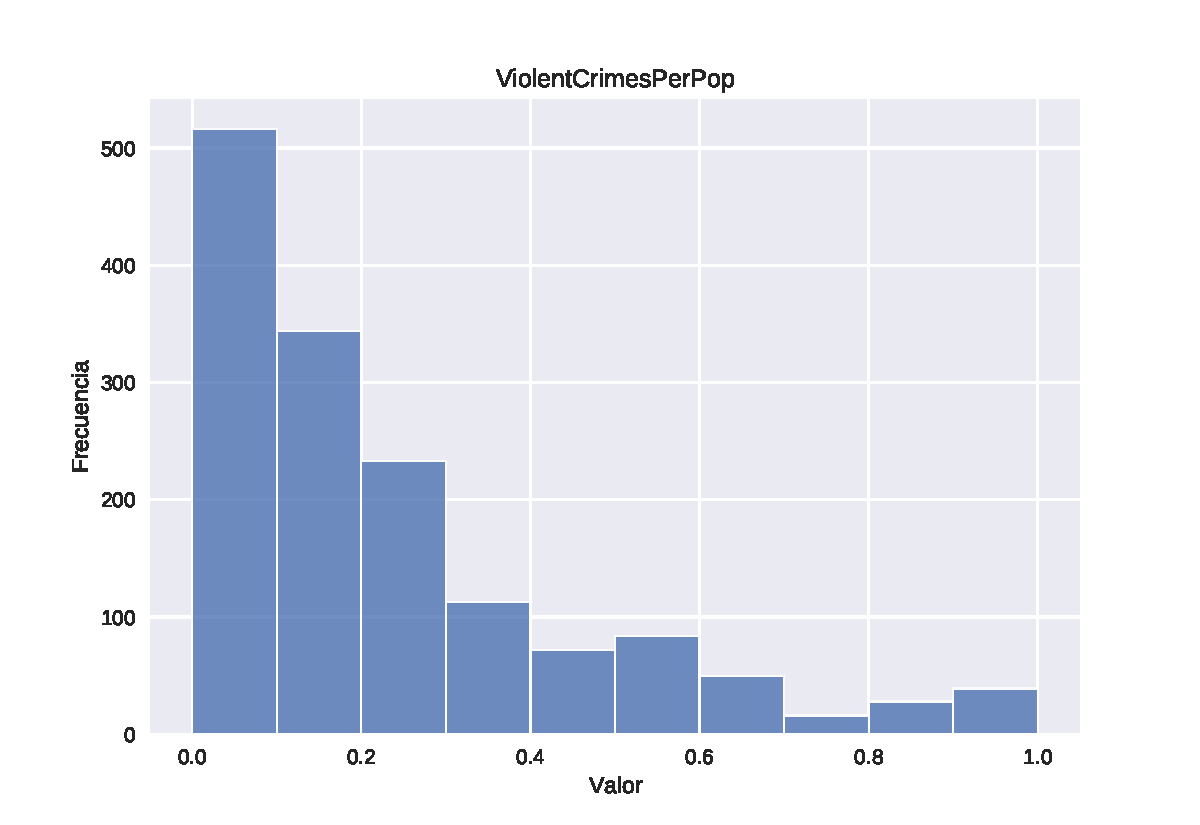
\includegraphics[width=\textwidth]{HistViolentCrimesPerPop}
    \caption{Distribución de la variable \texttt{ViolentCrimesPerPop}.}
    \label{fig:histVCPP}
\end{figure}

Continuamos obteniendo información sobre los valores perdidos, tendremos que tratar las variables que los contengan en el preprocesado y para ello debemos obtener cierta información sobre las mismas. En primer lugar, contamos el número de variables con valores perdidos: 23, que son:

\begin{lstlisting}
  OtherPerCap, LemasSwornFT, LemasSwFTPerPop, LemasSwFTFieldOps, LemasSwFTFieldPerPop, LemasTotalReq, LemasTotReqPerPop, PolicReqPerOffic, PolicPerPop, RacialMatchCommPol, PctPolicWhite, PctPolicBlack, PctPolicHisp, PctPolicAsian, PctPolicMinor, OfficAssgnDrugUnits, NumKindsDrugsSeiz, PolicAveOTWorked, PolicCars, PolicOperBudg, LemasPctPolicOnPatr, LemasGangUnitDeploy, PolicBudgPerPop.
\end{lstlisting}

El porcentaje de valores perdidos en cada una de ellas es de 84.002006\%, excepto para la variable \texttt{OtherPerCap} (ingresos per capita para individuos del grupo ``otros'')  que es de 0.050150\%.

%Proseguimos el análisis de los datos estudiando las correlaciones entre las variables. Esto nos permitirá encontrar dependencias lineales entre las diferentes variables y la variable a predecir, así como relaciones lineales entre las propias variables. No todas las relaciones entre variables serán de este tipo, pero no por ello deja de ser interesante estudiar las correlaciones.

%%%%%%%%%%%%%%%%%%%%%%%%%%%%%%%%%%%%%%%%%%%%%%%%%%%%%%%%%%%%%%%%%%%%%%%%
%% 2. Selección de las clase/s de funciones a usar. Identificar cuáles y porqué.
%%%%%%%%%%%%%%%%%%%%%%%%%%%%%%%%%%%%%%%%%%%%%%%%%%%%%%%%%%%%%%%%%%%%%%%%
\subsection{Clases de funciones}
% Combinaciones lineales, cuadráticas, etc... de las observaciones.
% Justificar su uso o por qué no se consideran necesarias.
% https://scikit-learn.org/stable/modules/generated/sklearn.preprocessing.PolynomialFeatures.html#sklearn.preprocessing.PolynomialFeatures
Para realizar la predicción utilizaremos una clase de funciones lineal en el vector de pesos $w$. Como no tenemos mucha información sobre cómo se comportan los datos y qué relaciones existen entre ellos, consideramos que limitarnos a la clase \[
\mathcal{H}_0 = \{w_0 + w_1x_1 +\cdots + w_Nx_N : w \in R^{N+1}\}
\]
que podría ser una primera opción natural, no será suficiente en este caso. Tenemos bastantes variables y podrían existir relaciones no lineales entre ellas. Además, combinaciones lineales de las variables podrían aportar más información que las variables por separado. Añadir complejidad a la clase de funciones nos permitirá aprovechar estas posibles relaciones no lineales entre las variables, si existieran. Es por esto, que la clase de funciones a utilizar es la de los polinomios de las variables de hasta orden 2.
 \[
\mathcal{H} = \left \{w_0 + w_1x_1 +\cdots + w_Nx_N + \sum_{i,j = 1}^Nw_{ij} x_ix_j\right\}.
\]
Notamos que aunque la clase de funciones sea cuadrática en las variables $x_i$, es lineal respecto a $w$.


%%%%%%%%%%%%%%%%%%%%%%%%%%%%%%%%%%%%%%%%%%%%%%%%%%%%%%%%%%%%%%%%%%%%%%%
%% 3. Fijar conjuntos de training y test que sean coherentes.
%%%%%%%%%%%%%%%%%%%%%%%%%%%%%%%%%%%%%%%%%%%%%%%%%%%%%%%%%%%%%%%%%%%%%%
\subsection{Conjuntos de \textit{training} y \textit{test}}
%% TRAINING → Subconjunto de los datos que se estudia, se
%% visualiza y a la que se le aplican los modelos.
%% VALIDACIÓN → Subconjunto de los datos que indica cuál es el
%% mejor modelo.
%% TEST → Subconjunto de los datos que proporciona el error
%% cometido.
%% Posibles particiones:
%% I Si se decide usar el conjunto Validación: 50% training, 25%
%% Validación y 25% test.
%% I Si no se decide usar el conjunto de Validación: 70%
%% training y 30% test u 80% training y 20% test.
% https://towardsdatascience.com/train-validation-and-test-sets-72cb40cba9e7

En este caso, tenemos un único conjunto de datos. Lo dividiremos en \training y \test, puesto que utilizaremos el error cometido en el conjunto de \test para poder realizar una estimación del error fuera de la muestra. El conjunto de entrenamiento contará con un 75\% de los ejemplos y el de \test con el 25\% restante. Necesitamos más información para entrenar el modelo y calcular los hiperparámetros que para el cálculo posterior del error.

Además, para la seleccion del modelo utilizaremos validación cruzada con 5 particiones diferentes. Entrenaremos 5 veces los diferentes modelos, cada una de las veces entrenando con un subconjunto del 80\% de los datos de \training y usando el 20\% restante para realizar la validación. De esta manera evitamos que el conjunto elegido para validación sea determinante a la hora de tomar nuestra decisión, evitando que aumente el sobreajuste.


%%%%%%%%%%%%%%%%%%%%%%%%%%%%%%%%%%%%%%%%%%%%%%%%%%%%%%%%%%%%%%%%%%%%%%%%
%% 4. Preprocesado los datos: codificación, normalización, proyección, etc. Es decir, todas las
%% manipulaciones sobre los datos iniciales hasta fijar el conjunto de vectores de caraterísticas
%% que se usarán en el entrenamiento.
%%%%%%%%%%%%%%%%%%%%%%%%%%%%%%%%%%%%%%%%%%%%%%%%%%%%%%%%%%%%%%%%%%%%%%%%
\subsection{Preprocesado}
%% ¿Por qué se preprocesan los datos?
%% Para eliminar impurezas y reducir la probabilidad de aprender de
%% manera errónea de los datos. Causas:
%% I Datos incompletos (Valores perdidos)
%% I Datos con ruido
%% I Datos inconsistentes
%% Tareas:
%% (esta lista es una sugerencia, por favor, elegid las que consideréis interesantes y/o necesarias)
%% I Colección, integración y transformación
%% Obtención de los datos, de una o más fuentes
%% Decodificación
%% Integración de datos de distintas bases de datos
%% Generación nuevo conocimiento
%% I Limpieza
%% - Modificación de datos con conflicto
%% - Eliminación de outliers
%% - Tratamiento de valores perdidos y problemas de ruido
%% I Reducción
%% - Selección de características
%% - Selección de instancias
%% - Discretización

Nos encontramos con un conjunto de 127 variables (más la variable a predecir) que ha sido previamente escalado al intervalo $[0,1]$. En primer lugar, se eliminarán las variables calificadas por los creadores de la base de datos como \textit{not predictive}. A continuación, se tratan las variables con valores perdidos, ya hemos visto que son 23.  

Para las variables que presenten valores perdidos se utilizará el siguiente criterio: si el porcentaje de valores desconocidos supera el 30\%, eliminaremos la variable, pues se considera que pasado el umbral la información que estaríamos añadiendo al problema sería demasiada y podría no coincidir con la realidad; en caso contrario, si el porcentaje de valores desconocidos es inferior al 30\%, se rellenarán estos valores mediante la técnica del vecino más cercano (\cite{}). Se barajó la opción de utilizar sustituir los valores perdidos por el valor medio para esta variable, pero esto provocaría errores grandes si nos las variables tuvieran ruido. Tras este paso, tendremos 100 de las variables originales.

Como la clase de funciones a utilizar, polinomios de las variables de hasta orden 2, añade nuevas características, pasamos de tener las 127 variables originales a tener 5151, lo que aumentará considerablemente el tiempo de cómputo. Además, como estas variables se han formado a partir de las originales, podrían, por un lado, resumir en una única variable información sobre dos de las originales, o, por otro lado, generar información redundante. Es por esto, que se procederá a seleccionar variables. Para seleccionar las variables más relevantes se utilizará la regularización LASSO, que dará un peso nulo a aquellas variables que no aporten mucha información para el proceso de aprendizaje (\cite{}). 

%%%%%%%%%%%%%%%%%%%%%%%%%%%%%%%%%%%%%%%%%%%%%%%%%%%%%%%%%%%%%%%%%%%%%%%%
%% 5. Fijar la métrica de error a usar. Discutir su idoneidad para el problema.
%%%%%%%%%%%%%%%%%%%%%%%%%%%%%%%%%%%%%%%%%%%%%%%%%%%%%%%%%%%%%%%%%%%%%%%%
\subsection{Métrica de error}
%% Elegir la métrica a usar y discutir su elección. Teniendo en cuenta
%% si se trata de un problema de regresión o de clasificación, así
%% como el tipo de problema a tratar.
%% I Regresión Aquí y Aquí
%% I Clasificación Aquí
Como nos encontramos ante un problema de regresión lineal, elegerimos la métrica de error usual en este tipo de problemas: error cuadrático medio. Para medir el error cometido al predecir el valor de las variables del conjunto $\{(x_1,y_1),\cdots,(x_n,y_n)\}$, donde $x_i$ es el vector de características e $y_i$ el verdadero valor de \textit{Per Capita Violent Crimes}, utilizando nuestra función hipótesis $h$, haremos:\[
E(h) = \frac{1}{n}\sum_{i=1}^n\left(y_i-h(x_i)\right)^2.
\]

%%%%%%%%%%%%%%%%%%%%%%%%%%%%%%%%%%%%%%%%%%%%%%%%%%%%%%%%%%%%%%%%%%%%%%%%
%% 8. Identificar los modelos a usar.
%%%%%%%%%%%%%%%%%%%%%%%%%%%%%%%%%%%%%%%%%%%%%%%%%%%%%%%%%%%%%%%%%%%%%%%%
\subsection{Modelos}
%% Posibles modelos a usar:
%% I Regresión lineal
%% I Regresión logística
%% I Perceptrón + Pocket
Por la naturaleza del problema, vamos a predecir una variable numérica en un intervalo, el modelo elegido es regresión lineal. No tendría sentido en este caso usar modelos como perceptrón o regresión logística, inherentes al problema de clasificación.

%%%%%%%%%%%%%%%%%%%%%%%%%%%%%%%%%%%%%%%%%%%%%%%%%%%%%%%%%%%%%%%%%%%%%%%%
%% 6. Discutir la técnica de ajuste elegida.
%%%%%%%%%%%%%%%%%%%%%%%%%%%%%%%%%%%%%%%%%%%%%%%%%%%%%%%%%%%%%%%%%%%%%%%%
\subsection{Técnica de ajuste}
%% Según modelo a usar, qué técnica de ajuste utilizas (SGD,
%% Pseudoinversa...) y razone por qué lo has elegido.

SGD por eficiencia, al haber aumentado el número de variables

%%%%%%%%%%%%%%%%%%%%%%%%%%%%%%%%%%%%%%%%%%%%%%%%%%%%%%%%%%%%%%%%%%%%%%%%
%% 7. Discutir la necesidad de regularización y en su caso la justificar la función usada para ello.
%%%%%%%%%%%%%%%%%%%%%%%%%%%%%%%%%%%%%%%%%%%%%%%%%%%%%%%%%%%%%%%%%%%%%%%%
\subsection{Regularización}
%% La regularización se trata del método que penaliza la complejidad
%% del modelo, al usar función de coste. Produciendo modelos más
%% simples que generalizan mejor.
%% I L1 (Regularización Lasso) → Interesante cuando se observa
%% que algunas de las características no influyen demasiado en
%% el modelo. Al dar coeficientes a cada atributo para generar
%% la combinación de ellas, ciertos coeficientes tenderán a 0.
%% Funciona mejor cuando los atributos no están correlados
%% entre sí.
%% I L2 (Regularización Ridge) → Útil cuando parezca que
%% varios de los atributos están correlados entre ellos.
%% Hace que los coeficientes sean pequeños.
%% Funciona mejor cuando la mayoría de los atributos son
%% relevantes.


%%%%%%%%%%%%%%%%%%%%%%%%%%%%%%%%%%%%%%%%%%%%%%%%%%%%%%%%%%%%%%%%%%%%%%%%
%% 9. Estimación de hiperparámetros y selección del mejor modelo.
%%%%%%%%%%%%%%%%%%%%%%%%%%%%%%%%%%%%%%%%%%%%%%%%%%%%%%%%%%%%%%%%%%%%%%%%
\subsection{Estimación de hiperparámetros y selección del mejor modelo}
%% 1. Ajustar los hiperparámetros del modelo.
%% 2. Ajustar los datos de validación (o test).
%% 3. Seleccionar el que se considera el mejor de los modelos y
%% argumentar por qué se elige.

%%%%%%%%%%%%%%%%%%%%%%%%%%%%%%%%%%%%%%%%%%%%%%%%%%%%%%%%%%%%%%%%%%%%%%%%
%% 10. Estimación por validación cruzada del error E out del modelo. Compárela con E test , ¿que
%% conclusiones obtiene?
%%%%%%%%%%%%%%%%%%%%%%%%%%%%%%%%%%%%%%%%%%%%%%%%%%%%%%%%%%%%%%%%%%%%%%%%
\subsection{Estimación del error}
%% Especificar el error que se produce al ajustar el modelo.

%%%%%%%%%%%%%%%%%%%%%%%%%%%%%%%%%%%%%%%%%%%%%%%%%%%%%%%%%%%%%%%%%%%%%%%%
%% 11. Suponga que Ud ha sido encargado de realizar este ajuste para una empresa. ¿Qué modelo
%% les propondría y que error E out les diría que tiene?. Justifique las decisiones.
%%%%%%%%%%%%%%%%%%%%%%%%%%%%%%%%%%%%%%%%%%%%%%%%%%%%%%%%%%%%%%%%%%%%%%%%
\subsection{Conclusiones}
%% Responder y argumentar:
%% I ¿Representa el modelo de manera adecuada los datos?
%% I ¿Consideras que la calidad del modelo es buena?
%% I ¿Es tu modelo el que proporciona el mejor error?
%% I ¿Por qué te has decidido por este modelo?
\newpage

%%%%%%%%%%%%%%%%%%%%%%%%%%%%
\printbibliography
% https://realpython.com/pandas-python-explore-dataset/
\end{document}
